\documentclass[12pt]{article}
\frenchspacing
\usepackage[utf8x]{inputenc}
\usepackage[T2A]{fontenc}
\usepackage{amsmath}
\usepackage{amsfonts}
\usepackage{amssymb}
\usepackage[russian]{babel}
\usepackage{graphicx}
\usepackage[left=2cm,right=2cm,top=2cm,bottom=2cm,bindingoffset=0cm]{geometry}
\author{Рашковецкий М.М., группа 526т}
\date{\today}
\title{Лабораторная работа 2.2.6\\Определение энергии активации по температурной зависимости вязкости жидкости}
\begin{document}
	\maketitle
	
	{\parindent=1cm \hangindent=1cm \parskip=0.5cm
	{\bfseries Цель работы:} измерение скорости падения шариков при разной температуре жидкости и вычисление вязкости жидкости по закону Стокса.
	
	\hangindent=1cm
	{\bfseries Оборудование и материалы:} стеклянный цилиндр с глицерином, термостат, секундомер, микроскоп, стеклянные и железные шарики.\par}
	\section*{Краткая теория}
	
	\indent Для перехода в новое состояние молекула жидкости должна преодолеть участки с высокой потенциальной энергией, которая больше тепловой, этим обусловена высокая вязкость жидкостей. Она обратно пропорциональна доле молекул, способных на этот переход, поэтому из распределения Больцмана
	\begin{equation}
	\label{eq:viscosity_temp}
	\eta \sim e^\frac{W}{kT},
	\end{equation}
	где $W$ --- энергия активации жидкости.
	
	По графику в координатах $\left( \frac{1}{T}, \ln \eta \right)$ можно найти $W$. Если график аппроксимирован как
	\begin{equation}
	\label{eq:exp_linearisation}
	\ln \eta = \frac{A}{T}+B,
	\end{equation}
	то энергия активации
	\begin{equation}
	\label{eq:act_energy_from_exp}
	W=kA.
	\end{equation}
	
	Формула \eqref{eq:viscosity_temp} даёт неплохое согласие при небольших разностях температур, но дальше становится плохо применимой, потому что выведена очень приближённо.
	
	Для ламинарного обтекания шарика бесконечной жидкостью верна формула Стокса:
	\begin{equation}
	\label{eq:stocks}
	\vec{F}=-6\pi \eta r\vec{v},
	\end{equation}
	где $r$ и $\vec{v}$ --- радиус и скорость шарика, $\vec{F}$ --- сила сопротивления, действуюбщая на него.
	
	Вопрос о применимости формулы \eqref{eq:stocks} решается только экспериментально. Критерием для этого может  служить число Рейнольдса
	\begin{equation}
	\label{eq:reinolds}
	Re=\frac{\rho vr}{\eta}.
	\end{equation}
	Если $Re<0{,}5$, то течение можно считать ламинарным.
	
	Для вертикального движения шарика в жидкости из второго закона Ньютона (на него действуют сила тяжести, сила Архимеда и сила сопротивления) в проекции на вертикальную ось легко получить следующее дифференциальное уравнение:
	\begin{equation}
	\label{eq:motion_diff_ur}
	Vg \left( \rho -\rho_\text{ж} \right) -6\pi \eta rv=V\rho \frac{dv}{dt},
	\end{equation}
	где $V$ --- объём шарика, $\rho$ и $\rho_\text{ж}$ --- плотности шарика и жидкости.
	
	Его решение имеет вид:
	\begin{equation}
	\label{eq:motion_diff_ur_sol}
	v=v_\text{уст}-\left( v_\text{уст}-v_0 \right) e^{-frac{t}{\tau}},
	\end{equation}
	где $v_0$ --- скорость в начальный момент времени,
	\begin{equation}
	\label{eq:v_ust}
	v_\text{уст}=\frac{Vg \left( \rho -\rho_\text{ж} \right)}{6\pi \eta r} = \frac{2}{9} gr^2 \frac{\rho -\rho_\text{ж}}{\eta}
	\end{equation}
	и
	\begin{equation}
	\label{eq:tau}
	\tau=\frac{V \rho}{6\pi \eta r} = \frac{2}{9} \frac{r^2\rho}{\eta}.
	\end{equation}
	
	Как видно из \eqref{eq:motion_diff_ur_sol}, скорость экспоненциально приближается к установившейся со временем релаксации $\tau$. При временах, в несколько раз превышающих время релаксации, процесс уже можно считать установившимся.
	
	Из \eqref{eq:v_ust} ясно, что если измерить на опыте $v_\text{уст}$, $r$, $\rho$ и $\rho_\text{ж}$, можно определить вязкость:
	\begin{equation}
	\label{eq:viscosity_from_exp}
	\eta=\frac{2}{9} gr^2 \frac{\rho -\rho_\text{ж}}{v_\text{уст}}.
	\end{equation}
	
	Есть два пути проверки применимости формулы Стокса:
	\begin{enumerate}
	\item Подсчёт числа Рейнольдса из \eqref{eq:reinolds} и \eqref{eq:viscosity_from_exp}:
	\begin{equation}
	\label{eq:reinolds_from_exp}
	Re=\frac{9 v_\text{уст}^2}{2gr} \frac{\rho}{\rho -\rho_\text{ж}}.
	\end{equation}
	\item Проверка отсутствия систематической зависимости $\eta$ от $r$.
	Если она наблюдается, можно использовать более точную формулу, учитывающую ограниченность жидкости в нашем эксперименте, полученную для движения шарика вдоль оси сосуда:
	\begin{equation}
	\label{eq:viscosity_from_exp_better}
	\eta=\frac{2}{9} gr^2 \frac{\rho -\rho_\text{ж}}{\left( 1 + 2{,}4 \frac{r}{R} \right) v_\text{уст}},
	\end{equation}
	где $R$ --- радиус сосуда.
	\end{enumerate}
	
	Также можно найти путь, пройденный шариком, проинтегрировав \eqref{eq:motion_diff_ur_sol}:
	\begin{equation}
	\label{eq:motion_dist}
	S = v_\text{уст} \tau \left( \frac{t}{\tau}-1+e^{-\frac{t}{\tau}} \right).
	\end{equation}
	
	Случаю установления $t \gg \tau$ соответствует
	\begin{equation}
	\label{eq:dist_gg}
	S \gg v_\text{уст} \tau = \frac{4gr^4 \rho \left( \rho -\rho_\text{ж} \right)}{81\eta^2}.
	\end{equation}
	
	Сделаем оценку сверху. В эксперименте $r < 1 \,\text{мм}$, $\rho < 8000\frac{\text{кг}}{\text{м}^3}$, $\rho_\text{ж} > 1000 \frac{\text{кг}}{\text{м}^3}$, $\eta > 0{,}05 \,\text{Па}\cdot \text{с}$, тогда
	\begin{equation}
	\label{eq:dist_gg_oc_up}
	S \gg 1,1 \,\text{см}.
	\end{equation}
	
	\section*{Установка}
	
	Установка состоит из сосуда С в рубашке, омываемового циркулирующей водой В из термостата Т. На термостате устанавливаются разные температуры, которые приобретает и глицерин в сосуде.
	
	\begin{figure}[h!]
	\caption{Схема установки}
	\label{fig:scheme}
	\begin{center}
	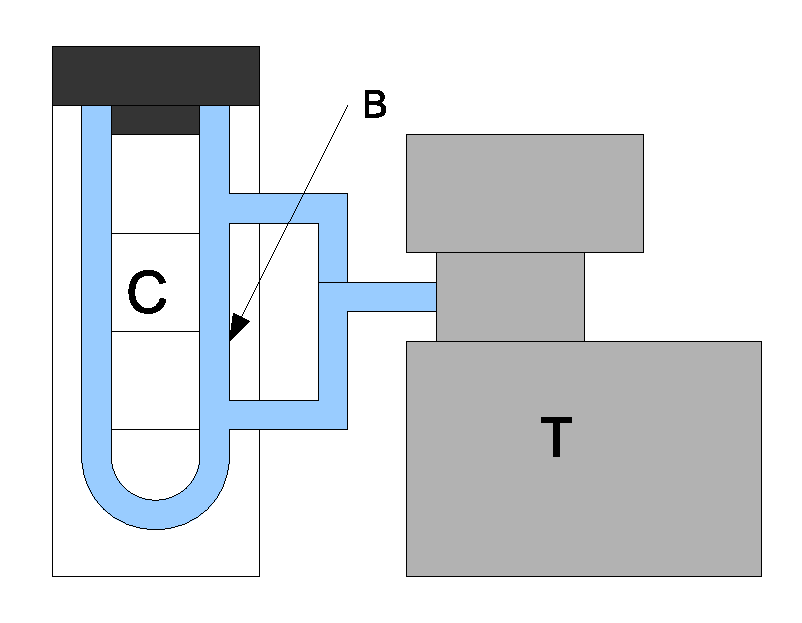
\includegraphics[scale=1]{scheme.eps}
	\end{center}
	\end{figure}
	
	Для шариков, сбрасываемых в сосуд, рекомендуется измерять несколько диаметров и усреднять, потому что они могут быть не вполне сферическими.
	
	\section*{Ход работы}
	
	\begin{enumerate}
	\item Мы отобрали 10 железных шариков ($\rho_\text{жел}=7800\frac{\text{кг}}{\text{м}^3}$) и 10 стеклянных ($\rho_\text{ст}=2500\frac{\text{кг}}{\text{м}^3}$).
	\item Измерили диаметр сосуда $D=2{,}4\,\text{см}$.
	\item Положив каждый из них под микроскоп в разных положениях по 3 раза, измерили по 3 разных диаметра.
	\item Выставили температуру $t$ на термостате, подождали, пока она установится. \label{exp_repeat_begin}
	\item Сбросили в сосуд по 2 железных и 2 стеклянных шарика, замерили время $\tau$, за которое каждый из них проходит расстояние между нижними полосами $l=10\,\text{см}$. \label{exp_repeat_end}
	\item Повторили пп. \ref{exp_repeat_begin} -- \ref{exp_repeat_end} для 5 разных температур.
	
	\end{enumerate}
	
	\section*{Обработка результатов}
	
	Результаты измерений приведены в таблице \ref{table:results_exp}. Плотность глицерина для нужных температур снята из графика в лабнике (хотя целесообразность этого весьма сомнительна --- изменения плотности крайне незначительны относительно погрешностей.)
	
	\begin{table}[h!]
	\caption{Результаты эксперимента}
	\label{table:results_exp}
	\begin{center}
	\begin{tabular}{|c|c|c|c|c|c|c|c|}
	\hline
	№ & \multicolumn{3}{c|}{$d_i$, мм} & $t, ^\circ \text{C}$ & $\tau$, с & $\rho, \text{кг}/ \text{м}^3$ & $\rho_\text{ж}, \text{кг}/ \text{м}^3$ \\
	\hline
	1 & 0,6 & 0,7 & 0,7 & 33 & 11,1 & 7800 & 1254 \\
	2 & 0,65 & 0,7 & 0,65 & 33 & 10,9 & 7800 & 1254 \\
	3 & 0,5 & 0,6 & 0,7 & 40 & 10,9 & 7800 & 1250 \\
	4 & 0,8 & 0,8 & 0,7 & 40 & 6,0 & 7800 & 1250 \\
	5 & 0,7 & 0,7 & 0,7 & 47 & 5,0 & 7800 & 1245 \\
	6 & 0,8 & 0,7 & 0,7 & 26 & 12,8 & 7800 & 1258 \\
	7 & 0,7 & 0,8 & 0,7 & 47 & 4,8 & 7800 & 1245 \\
	8 & 0,9 & 0,8 & 0,8 & 26 & 10,0 & 7800 & 1258 \\
	9 & 1,9 & 1,9 & 1,8 & 26 & 9,7 & 2500 & 1258 \\
	10 & 2,1 & 2,0 & 2,0 & 54 & 2,3 & 2500 & 1251 \\
	11 & 2,0 & 2,0 & 2,0 & 26 & 9,9 & 2500 & 1258 \\
	12 & 2,0 & 1,9 & 1,9 & 54 & 2,2 & 2500 & 1251 \\
	13 & 2,1 & 1,9 & 1,9 & 47 & 3,3 & 2500 & 1245 \\
	14 & 2,1 & 2,0 & 2,2 & 47 & 3,3 & 2500 & 1245 \\
	15 & 1,9 & 2,0 & 2,0 & 40 & 4,6 & 2500 & 1250 \\
	16 & 2,1 & 2,0 & 2,0 & 40 & 5,1 & 2500 & 1250 \\
	17 & 1,8 & 2,0 & 1,9 & 33 & 6,4 & 2500 & 1254 \\
	18 & 2,0 & 2,1 & 2,0 & 33 & 7,7 & 2500 & 1254 \\
	19 & 0,8 & 0,9 & 0,8 & 54 & 2,6 & 7800 & 1251 \\
	20 & 0,8 & 0,75 & 0,75 & 54 & 2,8 & 7800 & 1251 \\
	\hline
	\end{tabular}
	\end{center}
	\end{table}
	
	После этого я рассчитал средние значения и среднеквадратичные отклонения диаметров для всех шариков.
	
	Вязкость я находил согласно \eqref{eq:viscosity_from_exp}
	\begin{equation}
	\label{eq:viscosity_from_exp_working}
	\eta=\frac{2}{9} gr^2 t \frac{\rho -\rho_\text{ж}}{l}.
	\end{equation}
	
	Отсюда её погрешность
	\begin{equation}
	\label{eq:viscosity_from_exp_sigma}
	\sigma_\eta=\eta \sqrt{\left( 2\frac{\sigma_r}{r} \right)^2 \left( \frac{\sigma_t}{t} \right)^2},
	\end{equation}
	где погрешность времени $\sigma_t \approx 0{,}1$ с.
	
	Число Рейнольдса находил по \eqref{eq:reinolds_from_exp}.
	
	\begin{table}[h!]
	\caption{Результаты обработки}
	\label{table:results_obr}
	\begin{center}
	\begin{tabular}{|c|c|c|c|c|c|}
	\hline
	№ & $d$, мм & $t, ^\circ \text{C}$ & $\eta, \text{Па}\cdot \text{с}$ & $Re$ & $\eta', \text{Па}\cdot \text{с}$ \\
	\hline
	1 & $0.67\pm 0.05$ & 33 & $0.18\pm 0.02$ & 0,02 & $0.17\pm 0.02$  \\
	2 & $0.67\pm 0.02$ & 33 & $0.173\pm 0.012$ & 0,02 & $0.163\pm 0.011$ \\
	3 & $0.60\pm 0.08$ & 40 & $0.14\pm 0.04$ & 0,02 & $0.13\pm 0.04$ \\
	4 & $0.77\pm 0.05$ & 40 & $0.126\pm 0.016$ & 0,06 & $0.115\pm 0.015$ \\
	5 & 0.7 & 47 & $0.0874\pm 0.0017$ & 0,1 & $0.0825\pm 0.0016$ \\
	6 & $0.73\pm 0.05$ & 26 & $0.25\pm 0.03$ & 0,015 & $0.23\pm 0.03$ \\
	7 & $0.73\pm 0.05$ & 47 & $0.092\pm 0.011$ & 0,1 & $0.087\pm 0.011$ \\
	8 & $0.83\pm 0.05$ & 26 & $0.25\pm 0.03$ & 0,02 & $0.23\pm 0.03$ \\
	9 & $1.87\pm 0.05$ & 26 & $0.229\pm 0.012$ & 0,05 & $0.197\pm 0.010$ \\
	10 & $2.03\pm 0.05$ & 54 & $0.064\pm 0.004$ & 0,9 & $0.055\pm 0.004$ \\
	11 & 2 & 26 & $0.267\pm 0.003$ & 0,05 & $0.229\pm 0.002$ \\
	12 & $1.93\pm 0.05$ & 54 & $0.055\pm 0.004$ & 1 & $0.047\pm 0.003$ \\
	13 & $1.97\pm 0.09$ & 47 & $0.087\pm 0.009$ & 0,4 & $0.075\pm 0.008$ \\
	14 & $2.10\pm 0.08$ & 47 & $0.099\pm 0.008$ & 0,4 & $0.084\pm 0.007$ \\
	15 & $1.97\pm 0.05$ & 40 & $0.121\pm 0.006$ & 0,2 & $0.103\pm 0.005$ \\
	16 & $2.03\pm 0.05$ & 40 & $0.143\pm 0.007$ & 0,2 & $0.122\pm 0.006$ \\
	17 & $1.90\pm 0.08$ & 33 & $0.157\pm 0.014$ & 0,1 & $0.134\pm 0.011$ \\
	18 & $2.03\pm 0.05$ & 33 & $0.215\pm 0.010$ & 0,08 & $0.184\pm 0.009$ \\
	19 & $0.83\pm 0.05$ & 54 & $0.064\pm 0.008$ & 0,3 & $0.060\pm 0.007$ \\
	20 & $0.77\pm 0.03$ & 54 & $0.059\pm 0.004$ & 0,3 & $0.055\pm 0.004$ \\
	\hline
	\end{tabular}
	\end{center}
	\end{table}
	
	Числа Рейнольдса получилось в основном достаточно маленьким ($Re<0{,}5$), за исключением шариков 10 и 12, но я посчитал, что их влияние на лучшую прямую незначительно, и не стал исключать их из рассмотрения.
	
	Затем я построил график (рис. \ref{fig:graph}) в соответствии с \eqref{eq:exp_linearisation} и линейно аппроксимировал его по методу наименьших квадратов с учётом весов точек (из погрешностей).
	
	\begin{figure}[h!]
	\caption{График}
	\label{fig:graph}
	\begin{center}
	\includegraphics[scale=0.7]{graph.pdf}
	\end{center}
	\end{figure}
	
	Разброс точек показался мне большим, поэтому я пересчитал вязкость по \eqref{eq:viscosity_from_exp_better}:
	\begin{equation}
	\label{eq:viscosity_from_exp_better_working}
	\eta'=\frac{2}{9} gr^2 t \frac{\rho -\rho_\text{ж}}{\left( 1 + 2{,}4 \frac{r}{R} \right) l},
	\end{equation}
	влиянием поправочного к \eqref{eq:viscosity_from_exp_working} члена на погрешность пренебрёг. Числа Рейнольдса я пересчитал, но ситуация с ними существенно не изменилась, поэтому не привожу их в отчёте.
	
	По этим данным построил ещё один график (рис. \ref{fig:graph1}).
	
	\begin{figure}[h!]
	\caption{График с поправкой}
	\label{fig:graph1}
	\begin{center}
	\includegraphics[scale=1]{graph1.pdf}
	\end{center}
	\end{figure}
	
	Ситуация с точками несколько улучшилась (их погрешности не изменились относительно прошлого случая, но они стали ближе к прямой).
	
	Значение углового коэффициента прямой
	\begin{equation}
	\label{eq:angle_coeff}
	A = \left( 4760\pm 120 \right) \text{K}.
	\end{equation}
	
	Тогда, согласно \eqref{eq:act_energy_from_exp}, энергия активации
	\begin{equation}
	\label{eq:act_energy_res}
	W = \left( 6{,}57\pm 0{,}17 \right) \cdot 10^{-20} \text{Дж} = \left( 0{,}41\pm 0{,}01 \right) \text{эВ}.
	\end{equation}
	
	Зная молярную массу глицерина $\mu=92\frac{\text{г}}{\text{моль}}$, несложно пересчитать удельную энергию активации:
	\begin{equation}
	\label{eq:act_energy_by_mass}
	W = \left( 430\pm 10 \right) \frac{\text{кДж}}{\text{кг}}.
	\end{equation}
	Это приблизительно на порядок ниже удельной теплоты парообразования, что соответствует здравому смыслу.
	
	Погрешность может быть сильно занижена, потому что не учтён разброс точек при подсчёте погрешности углового коэффициента.
	
\end{document}
